% Set up the document
\documentclass{article}

% Page size
\usepackage[
    letterpaper,]{geometry}

% Lines between paragraphs
\setlength{\parskip}{\baselineskip}
\setlength{\parindent}{0pt}

% Math
\usepackage{mathtools}
\usepackage{amssymb}
\usepackage{commath}

% Math notation macros
\DeclareMathOperator*{\res}{Res}

\newcommand{\R}{\mathbb{R}}
\newcommand{\C}{\mathbb{C}}
\newcommand{\Z}{\mathbb{Z}}

\def\*#1{\mathbf{#1}}
\def\ti#1{\tilde{#1}}
\newcommand{\dadvd}[2]{\dfrac{\text{D} #1}{\text{D} #2}} % advective derivative

\newcommand{\fC}{\mathcal{C}} % fancy C
\newcommand{\fS}{\mathcal{S}} % fancy S
\newcommand{\tphi}{\tilde{\phi}}
\newcommand{\nhat}{\mathbf{\hat{n}}}
\newcommand{\rhat}{\mathbf{\hat{r}}}
\newcommand{\thetahat}{\boldsymbol{\hat{\theta}}}
\newcommand{\xhat}{\mathbf{\hat{x}}}
\newcommand{\yhat}{\mathbf{\hat{y}}}
\newcommand{\zhat}{\mathbf{\hat{z}}}
\newcommand{\omegavec}{\boldsymbol{\omega}}
\newcommand{\tauvec}{\boldsymbol{\tau}}
\newcommand{\dtauvec}{\boldsymbol{\delta \tau}}
\newcommand{\dFvec}{\boldsymbol{\delta} \mathbf{F}}
\newcommand{\dF}{\delta F}
\newcommand{\ds}{\delta s}
\newcommand{\dz}{\delta z}
\newcommand{\dtau}{\delta \tau}
\newcommand{\titau}{\tilde{\tau}}
\newcommand{\tidtau}{\delta \tilde{\tau}}
\newcommand{\tiz}{\tilde{z}}
\newcommand{\tix}{\tilde{x}}
\newcommand{\tiy}{\tilde{y}}

% Links
\usepackage{hyperref}

% Page numbers at top right
\usepackage{fancyhdr}
\pagestyle{fancy}
\fancyhf{}
\fancyhead[R]{\thepage}
\renewcommand\headrulewidth{0pt}

% Graphics
\usepackage{float}
\usepackage{graphicx}
\graphicspath{ {./img/} }

\begin{document}

\textbf{MATH 462 Assignment 11} \\
\textbf{Matt Wiens \#301294492} \\
\textbf{2020-04-11}

\textbf{103) Pipe flow.} (3 pages)
Review the notes from 3D Poiseuille pipe flow. The other exact solution
for this case is for flow in a pipe with an annulus cross-section, $S
\leq r \leq R$. The integration in $r$ now allows for keeping the singular term
at $r = 0$.

In addition to solving for the velocity $W(r)$, calculate the mass flux
and the global force balance. Be clear about all the signs in your shear
stress calculation---the cancellation you need is obvious, but the
understanding is in the proper tracing of the signs. Your presentation
of the stress terms will be paid special attention.

\textbf{Solution}

Just as in the lecture notes, we will assume the flow is steady and
axisymmetric. Using the incompressible Navier-Stokes equations, we
deduced in lecture that pressure is a function of $z$ only and that the
$z$-velocity $W$ is a function of $r$ only, such that
%
\begin{equation*}
    p_z = - \frac{\Delta p}{L}
    ,
\end{equation*}
%
where $L$ is the length of the pipe, and that
%
\begin{equation}
    \frac{1}{r} \del{r W^\prime(r)}^\prime = - \frac{\Delta p}{\mu L}
    \label{eq:1-1}
    ,
\end{equation}
%
where the prime symbols denote $r$ derivatives. By integrating~\eqref{eq:1-1}
twice, and in doing so being clever to multiply by $r$ before the
first integration and divide by $r$ before the second integration, we
find that the general solution for $W$ is given by
%
\begin{equation*}
    W(r) = - \frac{\Delta p}{4 \mu L} r^2 + c_1 \log r + c_2
    ,
\end{equation*}
%
where $c_1$ and $c_2$ are constants that we need to determine.

To determine the constants $c_1$ and $c_2$ we will invoke ``no-slip''
boundary conditions at the walls of the pipe, so that $W(S) = W(R) =
0$. These conditions give us that
%
\begin{equation*}
    - \frac{\Delta p}{4 \mu L} S^2 + c_1 \log S + c_2
    = - \frac{\Delta p}{4 \mu L} R^2 + c_1 \log R + c_2
    = 0
    .
\end{equation*}
%
This is a system of two equations in two unknowns which we can solve to
obtain (I used Maple here)
%
\begin{align*}
    c_1 &= \frac{\Delta p}{4 \mu L} \frac{R^2 - S^2}{\log\del{\frac{R}{S}}}, \\
    c_2 &= \frac{\Delta p}{4 \mu L} \frac{S^2 \log R - R^2 \log S}{\log\del{\frac{R}{S}}}
    .
\end{align*}
%
Hence, we can write the velocity $W$ as
%
\begin{align*}
    W(r) &= - \frac{\Delta p}{4 \mu L} r^2
        + \del{\frac{\Delta p}{4 \mu L} \frac{R^2 - S^2}{\log\del{\frac{R}{S}}}} \log r
        + \del{\frac{\Delta p}{4 \mu L} \frac{S^2 \log R - R^2 \log S}{\log\del{\frac{R}{S}}}} \\
         &= \frac{\Delta p}{4 \mu L} \del{S^2 - r^2 + \frac{(R^2 - S^2) \log\del{\frac{r}{S}}}{\log\del{\frac{R}{S}}}}
    .
\end{align*}
%
The simplification obtained in the second line of the above equation can
be obtained by adding zero in the form of
%
\begin{equation*}
    \frac{S^2 \log{S}}{\log\del{\frac{R}{S}}}
    - \frac{S^2 \log{S}}{\log\del{\frac{R}{S}}}
\end{equation*}
%
to the first line of the equation, and then the remaining steps in the
simplification are trivial.

Having determined an explicit formula for $W$, we can now calculate the
mass flux through the pipe with
%
\begin{align*}
    \text{mass flux}
        &= \rho_0 2 \pi \int_S^R W(r) r \dif r \\
        &= \frac{\pi \rho_0 \Delta p}{2 \mu L}
            \int_S^R
                \del{r S^2 - r^3 + r \frac{(R^2 - S^2) \log\del{\frac{r}{S}}}{\log\del{\frac{R}{S}}}}
            \dif r
        .
\end{align*}
%
There is quite a lot to evaluate in the integrand of the above equation,
so we'll do each term separately. For the first term we have
%
\begin{equation*}
    S^2  \int_S^R r \dif r = \frac{S^2 (R^2 - S^2)}{2}
    ;
\end{equation*}
%
for the second term,
%
\begin{equation*}
    \int_S^R r^3 \dif r = \frac{R^4 - S^4}{4}
    ;
\end{equation*}
%
and for the third term,
%
\begin{align*}
    \frac{R^2 - S^2}{\log\del{\frac{R}{S}}}
    \int_S^R r \log\del{\frac{r}{S}} \dif r
    &=
    \frac{R^2 - S^2}{\log\del{\frac{R}{S}}}
    \del{\frac{R^2}{4} \del{2 \log\del{\frac{R}{S}} - 1} + \frac{S^2}{4}}
    \\
    &= \frac{R^2 (R^2 - S^2)}{2} - \frac{(R^2 - S^2)^2}{\log\del{\frac{R}{S}}}
    .
\end{align*}
%
Hence, combining our results, we have
%
\begin{align*}
    \text{mass flux}
        &= \frac{\pi \rho_0 \Delta p}{2 \mu L}
            \del{
                \frac{S^2 (R^2 - S^2)}{2}
                - \frac{R^4 - S^4}{4}
                + \frac{R^2 (R^2 - S^2)}{2}
                - \frac{(R^2 - S^2)^2}{\log\del{\frac{R}{S}}}
            } \\
        &= \frac{\pi \rho_0 \Delta p}{8 \mu L}
            \del{
                R^4 - S^4
                - \frac{(R^2 - S^2)^2}{\log\del{\frac{R}{S}}}
            }
      .
\end{align*}
%
Moving forward to the shear stress, we need there to be a net zero force
in the $z$ direction at $r = S$ and $r = R$ and hence a shear stress to
balance the pressure force. Because the pressure force is in the
positive $z$ direction, the shear force should be in the negative $z$
direction. Calculating the general formula for the shear stress, we have
%
\begin{align*}
    \tauvec_\rhat
        &= \mu W^\prime(r) \zhat \\
        &= \frac{\Delta p}{4 L} \dod{}{r} \del{S^2 - r^2 + \frac{(R^2 - S^2) \log\del{\frac{r}{S}}}{\log\del{\frac{R}{S}}}} \zhat \\
        &= \frac{\Delta p}{4 L} \del{- 2 r + \frac{R^2 - S^2}{r \log\del{\frac{R}{S}}}} \zhat
        .
\end{align*}
%
Evaluating the stress at our boundary walls we have
%
\begin{align*}
    \eval[1]{\del{2 \pi r L \tauvec_\rhat}}_{r = R} - \eval[1]{\del{2 \pi r L \tauvec_\rhat}}_{r = S}
        &= \frac{\pi \Delta p}{2} \del{- 2 R^2 + \frac{R^2 - S^2}{\log\del{\frac{R}{S}}}} \zhat
           - \frac{\pi \Delta p}{2} \del{- 2 S^2 + \frac{R^2 - S^2}{\log\del{\frac{R}{S}}}} \zhat \\
        &= - \pi \Delta p (R^2 - S^2) \\
        &= - \text{pressure force}
        ,
\end{align*}
%
which is exactly what we would expect.

\newpage

\textbf{202) Complexification of torque.}
In this problem I'm going to do the following:
%
\begin{itemize}
    \item derive a formula for the torque about the origin due to forces on a body
    \item show an example of why an object in uniform flow is rotationally stable
    \item generalize the above example for general rotational stability
\end{itemize}

\textbf{Deriving the torque formula}

We're going to work in two dimensions here. Consider a fixed body which
has a closed contour $\fC$ (taken with counter-clockwise orientation) as
its boundary. Suppose we have a torque $\dtauvec$ about the origin due
to a force $\dFvec$ acting at some point $\*x$ which lies along a small
element $\ds$ of $\fC$. This torque is thus given by
%
\begin{equation}
    \dtau = (\*x \times \dFvec) \cdot \zhat = x \dF_y - y \dF_x
    \label{eq:tor-1}
    ,
\end{equation}
%
where for convenience we took $\dtau$ to be the $z$-component of
$\dtauvec$ (the other components are identically 0). Switching to complex
variables we will represent $\*x$ with $z = x + i y$ and $\dFvec$ with $\dF =
\dF_x + i \dF_y$. Note that we can now write~\eqref{eq:tor-1} as
%
\begin{equation}
    \dtau = \Re \cbr{z (\dF_y + i \dF_x)} = \Re \cbr{i z (\dF_x - i \dF_y)}
    \label{eq:tor-2}
    .
\end{equation}
%
Now that we've obtained the $\dF_x - i \dF_y$ term we essentially just
need to follow Acheson's steps for obtaining the Blasius integral
formula to get our desired equation for torque. For completeness, I will
reproduce these steps here (using the notation we've been using in
lectures).

Considering Figure $4.8$ in Acheson (p. 140), the net force on $\ds$ is
$(-p \sin \theta, p \cos \theta) \ds$ (where $p$ is the pressure acting
on $\ds$), and hence
%
\begin{equation}
    \dF_x - i \dF_y
        = \del{-p \sin \theta - i p \cos \theta} \ds = -p i e^{-i \theta} \ds
    \label{eq:tor-3}
    .
\end{equation}
%
Since $\fC$ is a streamline, we have that on $\fC$ (again, looking at the
Acheson figure is helpful)
%
\begin{align*}
    u = |\*u| \cos \theta, \\
    v = |\*u| \sin \theta.
\end{align*}
%
This lets us write, again on $\fC$,
%
\begin{equation}
    \dod{\Phi}{z} = u - i v = |\*u| e^{-i \theta}
    \label{eq:tor-4}
    .
\end{equation}
%
Using Bernouilli II (I think Bernoulli I would work as well because we
are on a streamline) we can express
%
\begin{equation}
    p = H_\infty - \frac{\rho_0}{2} |\*u|^2
    \label{eq:tor-5}
    ,
\end{equation}
%
on $\fC$, where $H_\infty$ is a constant, and so
substituting~\eqref{eq:tor-5} into~\eqref{eq:tor-3} give us
%
\begin{equation}
    \dF_x - i \dF_y
        = \del{\frac{\rho_0}{2} |\*u|^2 - H_\infty} i e^{-i \theta} \ds
    \label{eq:tor-6}
        .
\end{equation}
%
Now, using~\eqref{eq:tor-4}, we can further express~\eqref{eq:tor-6} as
%
\begin{equation}
    \dF_x - i \dF_y
        = i \frac{\rho_0}{2} \del{\dod{\Phi}{z}}^2 e^{i \theta} \ds - i e^{- i \theta} H_\infty \ds
    \label{eq:tor-7}
        .
\end{equation}
%
Now that we've obtained a suitable expression for $\dF_x - i \dF_y$,
we'll revisit~\eqref{eq:tor-2} and write
%
\begin{equation*}
    \dtau = \Re \cbr{
        i z \del{i \frac{\rho_0}{2} \del{\dod{\Phi}{z}}^2 e^{i \theta} \ds
        - i e^{- i \theta} H_\infty \ds}
    }
    .
\end{equation*}
%
Recognizing that $e^{i \theta} \ds = \dz$ we can write this in a ``cleaner form'' as
%
\begin{equation*}
    \dtau = \Re \cbr{
        i z \del{i \frac{\rho_0}{2} \del{\dod{\Phi}{z}}^2 \dz
        - i e^{- 2 i \theta} H_\infty \dz}
    }
    .
\end{equation*}
%
Dispensing with the ``real part'' notation for the moment, let us write
%
\begin{equation*}
    \tidtau =
        i z \del{i \frac{\rho_0}{2} \del{\dod{\Phi}{z}}^2 \dz
        - i e^{- 2 i \theta} H_\infty \dz}
    ,
\end{equation*}
%
and taking the limit as $\delta \to 0$, integrate along $\fC$ to obtain
%
\begin{equation*}
    \titau =
        \oint_\fC
        i z \del{i \frac{\rho_0}{2} \del{\dod{\Phi}{z}}^2 \dz
        - i e^{- 2 i \theta} H_\infty \dz}
    .
\end{equation*}
%
The second term in the integrand vanishes due to analyticity, leaving us
with the ``complexified'' torque formula
%
\begin{equation*}
    \titau =
    - \frac{\rho_0}{2} \oint_\fC z \del{\dod{\Phi}{z}}^2 \dif z
    .
\end{equation*}
%
Thus we have that
%
\begin{equation*}
    \tau = \Re \cbr{\titau} =
    - \frac{\rho_0}{2} \Re \cbr{\oint_\fC z \del{\dod{\Phi}{z}}^2 \dif z}
    .
\end{equation*}
%
As an aside, what does $\Im \cbr{\titau}$ represent? I don't have the
answer but I am curious.

\textbf{An example}

Now we'll consider the familiar flow past a circular cylinder whose
potential is given by
%
\begin{equation*}
    \Phi(z) = U_\infty \del{z + \frac{a^2}{z}}
\end{equation*}
%
(there's actually a figure for this with $U_\infty = 1$ and $a = 2$ in
my Milne-Thomson discussion below; Figure~\ref{fig:mt-2}). Now,
%
\begin{equation*}
    z \del{\dod{\Phi}{z}}^2
        = z \del{U_\infty - \frac{a^2}{z^2}}^2
        = z U_\infty^2 - \frac{2 U_\infty a^2}{z} + \frac{a^4}{z^2}
    ,
\end{equation*}
%
and so, denoting $\fC$ as the boundary of the cylinder (taken with a
counter-clockwise orientation) the net torque about the origin of the
cylinder is given by
%
\begin{align*}
    \tau
        &= - \frac{\rho_0}{2} \Re \cbr{\oint_\fC z \del{\dod{\Phi}{z}}^2 \dif z} \\
        &= - \frac{\rho_0}{2} \Re \cbr{2 \pi i\res_{z = 0} \cbr{z \del{\dod{\Phi}{z}}^2}} \\
        &= - \frac{\rho_0}{2} \Re \cbr{2 \pi i (-2 U_\infty a^2)} \\
        &= 0
     ,
\end{align*}
%
so the cylinder is rotationally stable, which makes sense.

\textbf{Generalizing the example}

What can we say about the torque about the origin for an arbitrary body?
The key lies in the circulation
%
\begin{equation*}
    \Gamma = \Re \cbr{\oint_\fC \dod{\Phi}{z} \dif z}
    .
\end{equation*}
%
The Laurent series for the above integrand, has a non-zero residue only if
the Laurent series for
%
\begin{equation*}
    z \del{\dod{\Phi}{z}}^2
\end{equation*}
%
also has a non-zero residue. Moreover, we can say that we have a non-zero
\textit{real} component of the residue for the integrand of the
circulation only if we have a non-zero real component of the
residue for the integrand of the torque integrand. Hence there is no net
torque about the origin only if the circulation around the body
is zero. (Whether the converse holds is non-trivial.)

\newpage

\textbf{203) Milne-Thomson circle theorem.}
In this problem I'm going to do the following:
%
\begin{itemize}
    \item describe what the Milne-Thomson circle theorem states
    \item prove the theorem
    \item show an example
    \item show another example (the ping pong ball in single/double hair dryer flow)
    \item explore whether we can extend this theorem to multiple circles
\end{itemize}

\textbf{The claim}

The claim here is that for any potential flow $\Phi$ whose singular
points lie in $|z| > a$, (i) we can preserve all singularities for $|z|
> a$, and (ii) have $|z| = a$ as a streamline with a new complex
potential
%
\begin{equation*}
    \Phi_{mt}(z) = \Phi(z) + \del{\Phi \del{\frac{a^2}{z^*}}}^*
    .
\end{equation*}

\textbf{Proof}

For notational convenience, denote
%
\begin{equation*}
    \ti{\Phi}(z) \coloneqq \del{\Phi \del{\frac{a^2}{z^*}}}^*
    .
\end{equation*}
%
To prove (i) we essentially need to show that there are no singularities
of $\ti\Phi$ after $|z| > a$. Suppose that $z$ is a singular point of
$\ti\Phi$. Then
%
\begin{equation*}
    \ti\Phi(z) = \del{\Phi \del{\frac{a^2}{z^*}}}^*
\end{equation*}
%
is a singularity. But since all singularities of $\Phi$ lie in $|z| >
a$ this implies that
%
\begin{equation*}
    \envert{\frac{a^2}{z^*}} > a
    ,
\end{equation*}
%
which further implies that $|z| < a$. Hence all singular points of
$\ti\Phi$ lie in $|z| < a$ and thus the singularities for $|z| > a$ for
$\Phi_{mt}$ are the same as for $\Phi$.

Now we'll prove (ii), which states that $|z| = a$ is a streamline. To
see this note that we can square the above expression to yield $z z^* =
a^2$. Then we have that, on $|z| = a$,
%
\begin{equation*}
    \ti\Phi(z)
        = \del{\Phi \del{\frac{a^2}{z^*}}}^*
        = \del{\Phi \del{\frac{(z z^*)}{z^*}}}^*
        = \del{\Phi(z)}^*
\end{equation*}
%
and thus (still on the $|z| = a$)
%
\begin{equation*}
    \Phi_{mt}(z) = \Phi(z) + \ti\Phi(z) = \Phi(z) + \del{\Phi(z)}^* = 2 \Re\del{\Phi(z)}
    .
\end{equation*}
%
Therefore $\Phi_{mt}(z)$ is purely real on the circle, and therefore
$\psi_{mt} = 0$ on $|z| = a$, and hence this is a streamline.

\textbf{An example}

Let's try this with a very simple example. Consider the potential
flow $\Phi(z) = z$. Here we have $\phi = x$ and $\psi = y$. This gives
us the familiar flow shown in Figure~\ref{fig:mt-1}.
%
\begin{figure}[ht]
    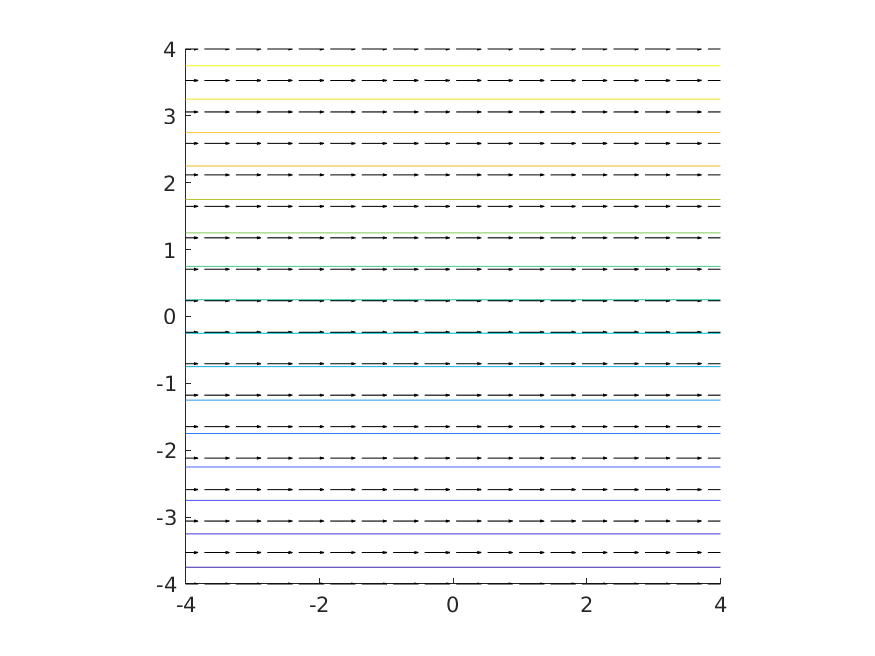
\includegraphics[width=35em]{mt_ex1_1}
    \centering
    \caption{Flow generated from $\Phi$}
    \label{fig:mt-1}
\end{figure}

Now let's see what happens when we apply Milne-Thomson, taking $a = 2$. This gives us
%
\begin{equation*}
    \Phi_{mt}(z) = z + \frac{4}{z}
    ,
\end{equation*}
%
and hence
%
\begin{align*}
    \phi_{mt} &= x + \frac{4 x}{x^2 + y^2}, \\
    \psi_{mt} &= y - \frac{4 y}{x^2 + y^2}
    .
\end{align*}
%
The resulting flow is plotted in Figure~\ref{fig:mt-2}. In this figure,
the streamline $\psi = 0$ is plotted in black, and we can see that it
aligns perfectly with the circle $|z| = 2$. Note also that velocity
quivers at $|z| < 2$ were not plotted, as this isn't part of the flow of
interest.
%
\begin{figure}[ht]
    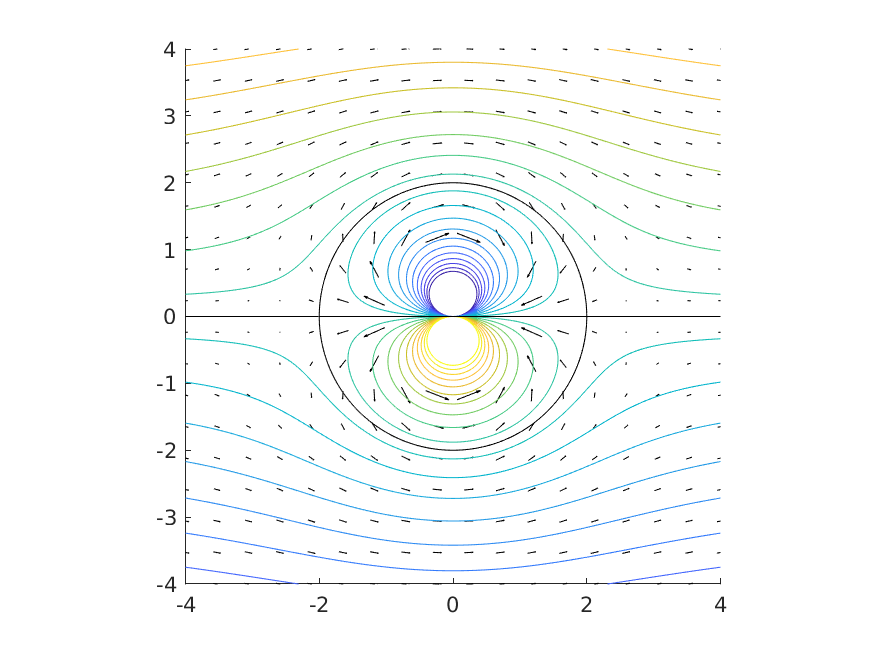
\includegraphics[width=35em]{mt_ex1_2}
    \centering
    \caption{Flow generated from $\Phi_{mt}$}
    \label{fig:mt-2}
\end{figure}

\textbf{Another example}

Now we'll look at the ``ping-pong ball in a hair dryer'' flow we briefly
looked at in lecture. For this example, we'll get a bit more involved in
the analysis than the previous example. First we'll look at ``double
hair dryer'' flow. Here, Milne-Thomson will essentially insert a circle
(our ping pong ball) into the centre of the double hair dryer
flow $\Phi$ given by
%
\begin{equation*}
    \Phi(z) = z^2
    .
\end{equation*}
%
Let's again apply Milne-Thomson, taking $a = 1$. This gives us
%
\begin{equation*}
    \Phi_{mt}(z) = z^2 + \frac{1}{z^2}
    .
\end{equation*}
%
Computing the real and imaginary components of $\Phi_{mt}$ then gives us
%
\begin{align*}
    \phi_{mt} &= \frac{x^2 - y^2}{(x^2 + y^2)^2} + x^2 - y^2, \\
    \psi_{mt} &= 2 x y - \frac{2 x y}{(x^2 + y^2)^2}
    .
\end{align*}
%
Plots of the double hair dryer flow generated from $\Phi$ and with the
embedded ping pong ball generated from $\Phi_{mt}$ are shown in
Figures~\ref{fig:mt-3} and~\ref{fig:mt-4}, respectively.
%
\begin{figure}[ht]
    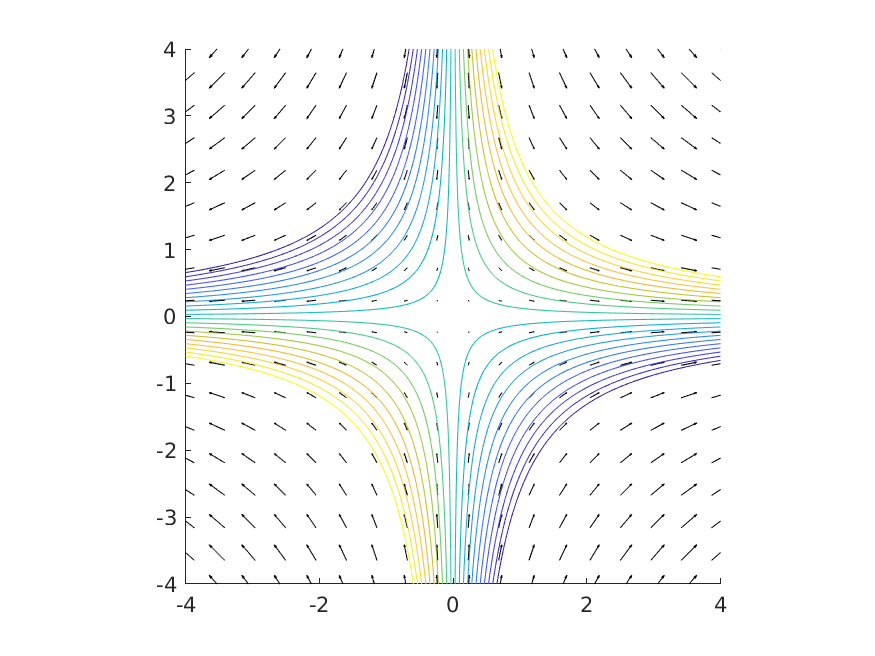
\includegraphics[width=35em]{mt_ex2_1}
    \centering
    \caption{Double hair dryer flow generated from $\Phi$}
    \label{fig:mt-3}
\end{figure}
%
\begin{figure}[ht]
    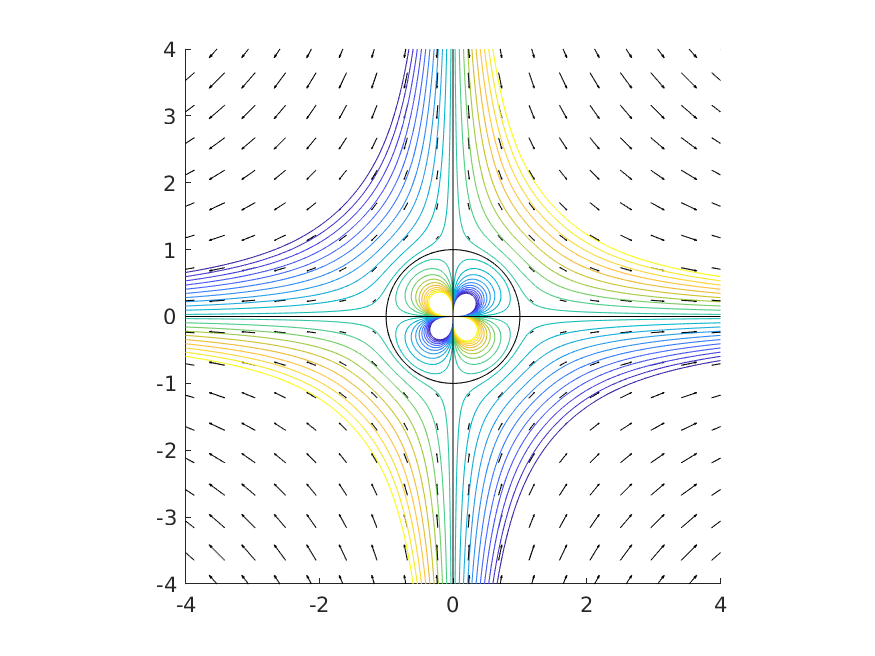
\includegraphics[width=35em]{mt_ex2_2}
    \centering
    \caption{Ping pong ball in double hair dryer flow generated from $\Phi_{mt}$}
    \label{fig:mt-4}
\end{figure}
%
We can calculate the force on the body using the Blasius integral
formula. First, we have that
%
\begin{equation*}
    \del{\Phi_{mt}^\prime(z)}^2
        = \del{2 z - \frac{2}{z^3}}^2
        = 4 x^2 - \frac{8}{x^2} + \frac{4}{x^6}
        ,
\end{equation*}
%
and, thus, using the residue theorem we have that
%
\begin{equation*}
    \*F_B \to \del{i \frac{\rho_0}{2} \oint_{\partial B} \del{\Phi_{mt}^\prime(z)}^2 \dif z}^* = 0
    .
\end{equation*}
%
Hence we would expect that a ping pong ball placed in the centre of the
double hair dryer flow will stay in the centre.

What if we offset the ping pong ball so it wasn't exactly in the centre
of the double hair dryer flow? Let's offset the ball by $\Delta x =
0.1$ units (horizontally to the right). We can model this by generating a
new potential $\Phi_{mt2}$ given by
%
\begin{equation*}
    \Phi_{mt2}(z) = (z + 0.1)^2 + \del{\frac{1}{z} + 0.1}^2
\end{equation*}
%
with real and imaginary components given by
%
\begin{align*}
    \phi_{mt2} &= \frac{x^2 - y^2}{(x^2 + y^2)^2} + \frac{0.2 x}{x^2 + y^2} + x^2 + 0.2x - y^2 + 0.02, \\
    \psi_{mt2} &= - \frac{2 x y}{(x^2 + y^2)^2} - \frac{0.2 y}{x^2 + y^2} + 2 x y + 0.2 y
    .
\end{align*}
%
This is shown in Figure~\ref{fig:mt-5} (since the offset is small,
the differences between this plot and Figure~\ref{fig:mt-4} are
small).
%
\begin{figure}[ht]
    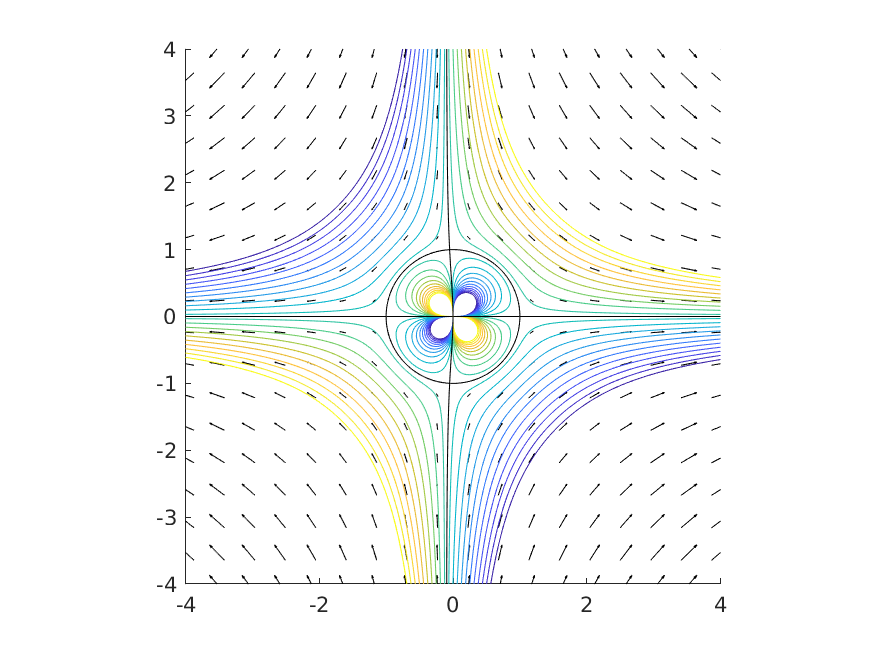
\includegraphics[width=35em]{mt_ex2_3}
    \centering
    \caption{Ping pong ball in hair dryer with offset flow generated from $\Phi_{mt2}$}
    \label{fig:mt-5}
\end{figure}
%
Let's go ahead and compute the Blasius integral formula again. First
we'll calculate the integrand in the Blasius integral formula:
%
\begin{equation*}
    \del{\Phi^\prime_{mt2}}^2
        = \del{0.2 - \frac{2}{z^3} - \frac{0.2}{z^2} + 2 z}^2
        = \frac{4}{z^6} + \frac{0.8}{z^5} + \frac{0.04}{z^4} - \frac{0.08}{z^3} - \frac{8.08}{z^2} - \frac{0.8}{z} + 0.04 + 0.8 z + 4 z^2
        .
\end{equation*}
%
Hence we have that
%
\begin{align*}
    \*F_B
        &\to \del{i \frac{\rho_0}{2} \oint_{\partial B} \del{\Phi_{mt2}^\prime(z)}^2 \dif z}^* \\
        &= \del{i \frac{\rho_0}{2} 2 \pi i \res_{z = 0} \sbr{\del{\Phi^\prime_{mt2}}^2}}^* \\
        &= \del{i \frac{\rho_0}{2} 2 \pi i (-0.8)}^* \\
        &= 0.8 \rho_0 \pi
    .
\end{align*}
%
So it would appear that the ping bong ball is being pushed away from the
centre of the double hair dryer flow with this offset.

Before moving on to the single hair dryer flow, let's consider any offset
$\tiz \in \C$ and see whether the centre of the flow is stable with
respect to this offset. In this case, our potential $\Phi_{mt3}$ will be
given by
%
\begin{equation*}
    \Phi_{mt3}(z) = (z + \tiz)^2 + \del{\frac{1}{z} + \tiz}^2
    .
\end{equation*}
%
Expressing $\tiz = \tix + i \tiy$ we have that (omitting the whole
calculation for brevity; the steps are identical to what we did with the
$\Delta x = 0.1$ horizontal offset)
%
\begin{equation*}
    \res_{z = 0} \del{\Phi^\prime_{mt3}}^2 = -8 (\tix + i \tiy)
    ,
\end{equation*}
%
and so
%
\begin{align*}
    \*F_B
        &\to \del{i \frac{\rho_0}{2} \oint_{\partial B} \del{\Phi_{mt3}^\prime(z)}^2 \dif z}^* \\
        &= \del{i \frac{\rho_0}{2} 2 \pi i \res_{z = 0} \sbr{\del{\Phi^\prime_{mt3}}^2}}^* \\
        &= \del{i \frac{\rho_0}{2} 2 \pi i (- 8 (\tix + i \tiy)}^* \\
        &= 8 \rho_0 \pi (\tix - i \tiy)
    .
\end{align*}
%
From this we can conclude that any perturbation of the ping pong ball
from the centre of the hair dryer flow will push the ping pong ball
\textit{away} from the centre in the horizontal direction and
\textit{towards} the centre in the vertical direction. Looking again at
the flow in Figure~\ref{fig:mt-3}, this result makes sense.

We've looked at the double hair dryer flow, but what can we say about
single hair dryer flow? It turns out that if we take the single hair
dryer flow to be a vertically translated version of our double hair
dryer flow, then we've already solved the problem. Considering our
generalization above, the ping pong ball is \textit{never} stable in the
centre of the single hair dryer flow. The ball will move vertically up
no matter what, and, if not horizontally centered, will also move
horizontally outwards. This is consistent with Figure~\ref{fig:mt-3}.
However, it is not consistent with the demo we saw in lecture, which
implies that this flow is not suitable to model the physics seen in the
lecture demo.

\textbf{Modelling multiple circles}

In our first example we showed how to embed a circle into the potential
flow $\Phi(z) = z$ to generate the new potential (this time taking $a = 1/2$)
%
\begin{equation*}
    \Phi_{mt}(z) = z + \frac{1}{4 z}
    .
\end{equation*}
%
However we can introduce \textit{another} circle into this flow by
offsetting this potential by $1$ unit and introducing another circle at the
origin of this new flow. We'll call this new flow $\Psi$ and, with the
second circle (again with $a = 1/2$) embedded into it, $\Psi_{mt}$. We
will thus take $\Psi$ to be given by
%
\begin{equation*}
    \Psi(z) = (z - 1) + \frac{1}{4 (z - 1)}
\end{equation*}
%
and hence $\Psi_{mt}$ is given by
%
\begin{equation*}
    \Psi_{mt}(z)
        = (z - 1) + \frac{1}{4 (z - 1)}
        + \del{\frac{1}{4z} - 1} + \frac{1}{4 (\frac{1}{4z} - 1)}
        .
\end{equation*}
%
This potential has real and imaginary components that are long and not
particularly informative, So I'm just going to use Maple to compute them
and use those results directly in my MATLAB code. The result is shown in
Figure~\ref{fig:mt-6}.
%
\begin{figure}[ht]
    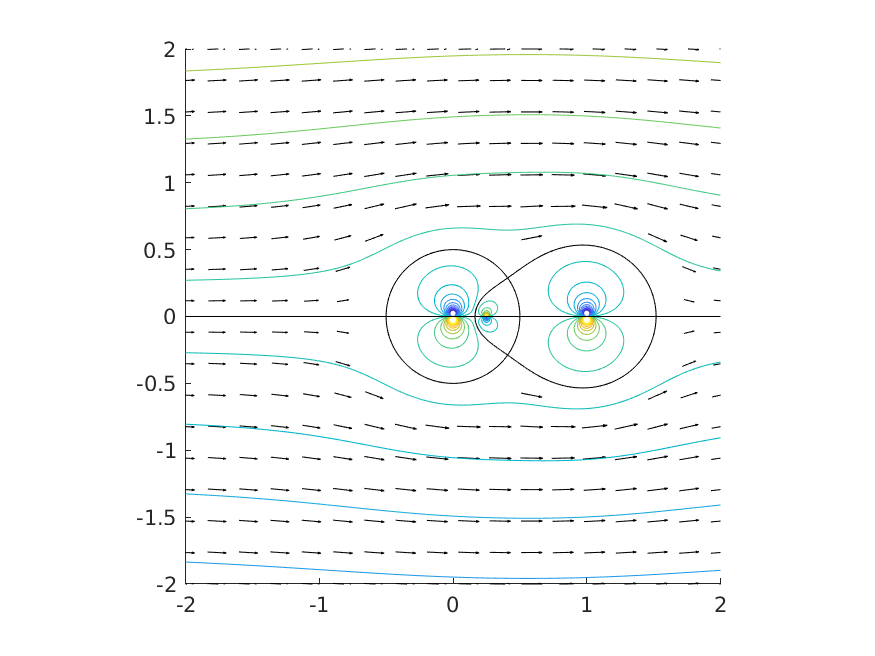
\includegraphics[width=35em]{mt_ex3_1}
    \centering
    \caption{Modelling two circle flow generated from $\Psi_{mt}$}
    \label{fig:mt-6}
\end{figure}
%
This result is physically plausible in that it looks roughly like what I
would expect to happen if we inserted two circles into the flow $\Phi$.

These circles are ``touching'' each other by design. What if they were
farther apart. Let's see what happens in this case. Here we will keep $a
= 1/2$ for both circles and offset horizontally $5$ units. This gives us
the final potential (after both circles are embedded)
%
\begin{equation*}
    \Psi_{mt2}
        = (z - 5) + \frac{1}{4 (z - 5)}
        + \del{\frac{1}{4z} - 5} + \frac{1}{4 (\frac{1}{4z} - 5)}
\end{equation*}
%
which results in the flow in Figure~\ref{fig:mt-7}.
%
\begin{figure}[ht]
    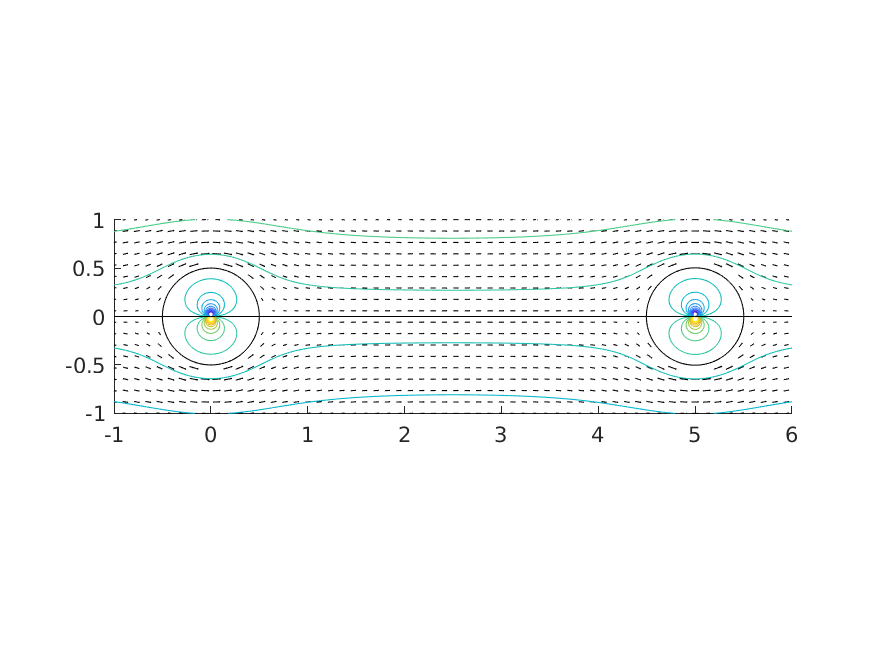
\includegraphics[width=35em]{mt_ex3_2}
    \centering
    \caption{Modelling two circle flow generated from $\Psi_{mt2}$}
    \label{fig:mt-7}
\end{figure}
%
Again, the results here look perfectly reasonable.

Based on these two example my conjecture is that, for any given flow, we
can approximate embedding \textit{any} object into the flow by
approximating it with non-overlapping circles and applying Milne-Thomson
successively in the manner we've done here.

\end{document}
